\documentclass{article}

% required 
\usepackage[hyphens]{url} % this wraps my URL versus letting it spill across the page, a bad habit LaTeX has

\usepackage{Sweave}
\usepackage{graphicx}
\usepackage{tabularx}
\usepackage{longtable}
\usepackage{natbib}
\usepackage{amsmath}
\usepackage{textcomp}%amoung other things, it allows degrees C to be added
\usepackage{float}
\usepackage[utf8]{inputenc} % allow funny letters in citaions 
\usepackage[nottoc]{tocbibind} %should add Refences to the table of contents?
\usepackage{amsmath} % making nice equations 
\usepackage{listings} % add in stan code
\usepackage{xcolor}
\usepackage{capt-of}%alows me to set a caption for code in appendix 
\usepackage[export]{adjustbox} % adding a box around a map
\usepackage{lineno}
\linenumbers
% recommended! Uncomment the below line and change the path for your computer!
% \SweaveOpts{prefix.string=/Users/Lizzie/Documents/git/teaching/demoSweave/Fig.s/demoFig, eps=FALSE} 
%put your Fig.s in one place! Also, note that here 'Fig.s' is the folder and 'demoFig' is what each 
% Fig. produced will be titled plus its number or label (e.g., demoFig-nqpbetter.pdf')
% make your captioning look better
\usepackage[small]{caption}
\usepackage{xr-hyper} %refer to Fig.s in another document
\usepackage{hyperref}

\setlength{\captionmargin}{30pt}
\setlength{\abovecaptionskip}{0pt}
\setlength{\belowcaptionskip}{10pt}

% optional: muck with spacing
\topmargin -1.5cm        
\oddsidemargin 0.5cm   
\evensidemargin 0.5cm  % same as oddsidemargin but for left-hand pages
\textwidth 15.59cm
\textheight 21.94cm 
% \renewcommand{\baselinestretch}{1.5} % 1.5 lines between lines
\parindent 0pt		  % sets leading space for paragraphs
% optional: cute, fancy headers
\usepackage{fancyhdr}
\pagestyle{fancy}
\fancyhead[LO]{Draft early 2022}
\fancyhead[RO]{Temporal Ecology Lab}
% more optionals! %

%%% end preambling. %%%

\begin{document}
\Sconcordance{concordance:traitsCG.tex:traitsCG.Rnw:%
1 57 1 1 17 14 0 3 3 1 17 14 0 1 3 2 1 1 17 14 0 1 3 1 17 14 0 1 3 2 1 %
1 17 14 0 1 3 1 17 14 0 1 3 1 17 14 0 1 3 2 1 1 17 14 0 1 3 2 1}


\section*{Running Cat's models}

\subsection*{Specific leaf area}
% latex table generated in R 3.6.3 by xtable 1.8-4 package
% Tue Nov 22 17:34:31 2022
\begin{table}[ht]
\centering
\caption{Summary of the intercept only model for SLA in 2019 (n = 599) with species (n = 18) and population (n = 5).} 
\begin{tabular}{rrrrrr}
  \hline
 & mean & 25\% & 75\% & n\_eff & Rhat \\ 
  \hline
alpha & 22.22 & -3.85 & 48.51 & 3272.72 & 1.00 \\ 
  mu\_a\_sp & 0.52 & -22.76 & 23.83 & 3982.78 & 1.00 \\ 
  sigma\_a\_sp & 29.60 & 11.85 & 41.73 & 4131.24 & 1.00 \\ 
  sigma\_a\_pop & 0.88 & 0.24 & 1.05 & 2095.84 & 1.00 \\ 
  sigma\_y & 9.03 & 8.84 & 9.20 & 6772.40 & 1.00 \\ 
  \end{tabular}
\end{table}
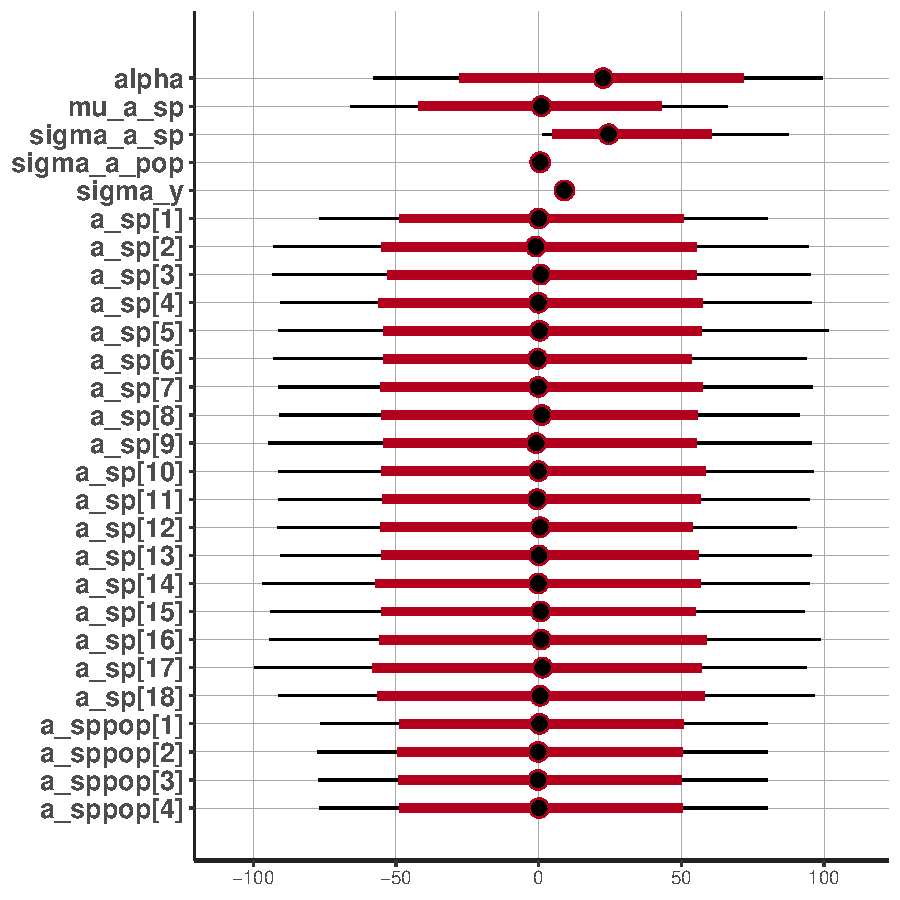
\includegraphics{traitsCG-fig3}

% latex table generated in R 3.6.3 by xtable 1.8-4 package
% Tue Nov 22 17:34:32 2022
\begin{table}[ht]
\centering
\caption{Summary of the intercept only model for SLA in 2022 (n = 446) with species (n = 13) and population (n = 5).} 
\begin{tabular}{rrrrrr}
  \hline
 & mean & 25\% & 75\% & n\_eff & Rhat \\ 
  \hline
alpha & 21.23 & -3.33 & 45.37 & 2283.14 & 1.00 \\ 
  mu\_a\_sp & -0.35 & -24.51 & 23.35 & 2224.31 & 1.00 \\ 
  sigma\_a\_sp & 5.53 & 0.90 & 6.03 & 1582.09 & 1.00 \\ 
  sigma\_a\_pop & 1.12 & 0.28 & 1.26 & 1415.77 & 1.00 \\ 
  sigma\_y & 6.96 & 6.80 & 7.11 & 4515.33 & 1.00 \\ 
  \end{tabular}
\end{table}\newpage

\subsection*{Leaf dry matter content}
% latex table generated in R 3.6.3 by xtable 1.8-4 package
% Tue Nov 22 17:34:33 2022
\begin{table}[ht]
\centering
\caption{Summary of the intercept only model for LDMC in 2019 (n = 599) with species (n = 18) and population (n = 5).} 
\begin{tabular}{rrrrrr}
  \hline
 & mean & 25\% & 75\% & n\_eff & Rhat \\ 
  \hline
alpha & 21.23 & -3.33 & 45.37 & 2283.14 & 1.00 \\ 
  mu\_a\_sp & -0.35 & -24.51 & 23.35 & 2224.31 & 1.00 \\ 
  sigma\_a\_sp & 5.53 & 0.90 & 6.03 & 1582.09 & 1.00 \\ 
  sigma\_a\_pop & 1.12 & 0.28 & 1.26 & 1415.77 & 1.00 \\ 
  sigma\_y & 6.96 & 6.80 & 7.11 & 4515.33 & 1.00 \\ 
  \end{tabular}
\end{table}
% latex table generated in R 3.6.3 by xtable 1.8-4 package
% Tue Nov 22 17:34:33 2022
\begin{table}[ht]
\centering
\caption{Summary of the intercept only model for LDMC in 2022 (n = 446) with species (n = 13) and population (n = 5).} 
\begin{tabular}{rrrrrr}
  \hline
 & mean & 25\% & 75\% & n\_eff & Rhat \\ 
  \hline
alpha & 21.23 & -3.33 & 45.37 & 2283.14 & 1.00 \\ 
  mu\_a\_sp & -0.35 & -24.51 & 23.35 & 2224.31 & 1.00 \\ 
  sigma\_a\_sp & 5.53 & 0.90 & 6.03 & 1582.09 & 1.00 \\ 
  sigma\_a\_pop & 1.12 & 0.28 & 1.26 & 1415.77 & 1.00 \\ 
  sigma\_y & 6.96 & 6.80 & 7.11 & 4515.33 & 1.00 \\ 
  \end{tabular}
\end{table}\newpage

\subsection*{Height}
% latex table generated in R 3.6.3 by xtable 1.8-4 package
% Tue Nov 22 17:34:34 2022
\begin{table}[ht]
\centering
\caption{Summary of the intercept only model for plant height in 2019 (n = 302) with species (n = 18) and population (n = 5).} 
\begin{tabular}{rrrrrr}
  \hline
 & mean & 25\% & 75\% & n\_eff & Rhat \\ 
  \hline
alpha & 1.26 & -20.15 & 22.84 & 2805.38 & 1.00 \\ 
  mu\_a\_sp & -0.34 & -21.96 & 21.13 & 2811.38 & 1.00 \\ 
  sigma\_a\_sp & 0.64 & 0.12 & 0.55 & 1005.87 & 1.00 \\ 
  sigma\_a\_pop & 0.65 & 0.12 & 0.55 & 1054.36 & 1.00 \\ 
  sigma\_y & 0.55 & 0.54 & 0.57 & 6267.25 & 1.00 \\ 
  \end{tabular}
\end{table}
% latex table generated in R 3.6.3 by xtable 1.8-4 package
% Tue Nov 22 17:34:37 2022
\begin{table}[ht]
\centering
\caption{Summary of the intercept only model for plant height in 2021 (n = 257) with species (n = 16) and population (n = 5).} 
\begin{tabular}{rrrrrr}
  \hline
 & mean & 25\% & 75\% & n\_eff & Rhat \\ 
  \hline
alpha & 2.74 & -18.60 & 24.61 & 3564.99 & 1.00 \\ 
  mu\_a\_sp & -0.01 & -21.64 & 21.83 & 3547.77 & 1.00 \\ 
  sigma\_a\_sp & 4.22 & 0.79 & 4.37 & 1336.33 & 1.00 \\ 
  sigma\_a\_pop & 0.58 & 0.13 & 0.60 & 1114.62 & 1.00 \\ 
  sigma\_y & 1.41 & 1.37 & 1.45 & 7806.45 & 1.00 \\ 
  \end{tabular}
\end{table}
% latex table generated in R 3.6.3 by xtable 1.8-4 package
% Tue Nov 22 17:34:38 2022
\begin{table}[ht]
\centering
\caption{Summary of the intercept only model for plant height in 2022 (n = 240) with species (n = 14) and population (n = 5).} 
\begin{tabular}{rrrrrr}
  \hline
 & mean & 25\% & 75\% & n\_eff & Rhat \\ 
  \hline
alpha & 3.05 & -19.58 & 25.59 & 2009.90 & 1.00 \\ 
  mu\_a\_sp & -0.15 & -22.67 & 22.44 & 2019.33 & 1.00 \\ 
  sigma\_a\_sp & 2.31 & 0.45 & 2.80 & 957.30 & 1.00 \\ 
  sigma\_a\_pop & 1.13 & 0.24 & 1.28 & 995.85 & 1.01 \\ 
  sigma\_y & 1.72 & 1.66 & 1.77 & 4029.93 & 1.00 \\ 
  \end{tabular}
\end{table}\newpage

\subsection*{Stem specific density}
% latex table generated in R 3.6.3 by xtable 1.8-4 package
% Tue Nov 22 17:34:39 2022
\begin{table}[ht]
\centering
\caption{Summary of the intercept only model for plant SSD in 2022 (n = 240) with species (n = 14) and population (n = 5).} 
\begin{tabular}{rrrrrr}
  \hline
 & mean & 25\% & 75\% & n\_eff & Rhat \\ 
  \hline
alpha & 2.06 & -26.84 & 32.81 & 276.07 & 1.01 \\ 
  mu\_a\_sp & -3.51 & -32.03 & 24.16 & 292.76 & 1.01 \\ 
  sigma\_a\_sp & 40.00 & 15.98 & 56.32 & 609.38 & 1.01 \\ 
  sigma\_a\_pop & 0.01 & 0.00 & 0.02 & 638.44 & 1.00 \\ 
  sigma\_y & 0.09 & 0.08 & 0.09 & 574.88 & 1.00 \\ 
  \end{tabular}
\end{table}

\end{document}
